%%%%%%%%%%%%%%%%%%%%%%%%%%%%%%%%%%%%%%%%%%%%%%%%%%%%%%%%%%%%%%%%%%%%%%%%%%%%%%%%%%
\begin{frame}[fragile]\frametitle{}
\begin{center}
{\Large sadhanpaad साधनपाद}
\end{center}
\end{frame}


%%%%%%%%%%%%%%%%%%%%%%%%%%%%%%%%%%%%%%%%%%%%%%%%%%%%%%%%%%%
\begin{frame}[fragile]\frametitle{Introduction}


	\begin{itemize}
	\item Sadhana in Sanskrit means `practice' and Sadhana Pada simply means, `the path of practice'. 	\item Here, in the second chapter of the Yoga Sutras, Patanjali explains the two paths or the two forms of Yoga: Kriya Yoga (क्रिया योग)and Ashtanga Yoga (Eightfold or Eight-limbed Yoga)
	\end{itemize}

\end{frame}

%%%%%%%%%%%%%%%%%%%%%%%%%%%%%%%%%%%%%%%%%%%%%%%%%%%%%%%%%%%
\begin{frame}[fragile]\frametitle{Kriya Yoga}


	\begin{itemize}
	\item The yoga of action, which consists of deliberate effort, a study of the self and traditional texts, and devotion. 
	\item The purpose of Kriya Yoga is to alleviate the causes of suffering and to attain Samadhi. 
	\item Kriya Yoga has three parts:
		\begin{itemize}
		\item Tapas – Endurance and Acceptance.
		\item Swadhyaaya – Self-awareness, and self-study.
		\item Ishwara Pranidhaana – Devotion to and love for the divine.
		\end{itemize}	
	\end{itemize}

\end{frame}

%%%%%%%%%%%%%%%%%%%%%%%%%%%%%%%%%%%%%%%%%%%%%%%%%%%%%%%%%%%
\begin{frame}[fragile]\frametitle{Ashtanga  Yoga}

A systematic and practical set of yogic knowledge divided into eight basic parts.

\begin{center}
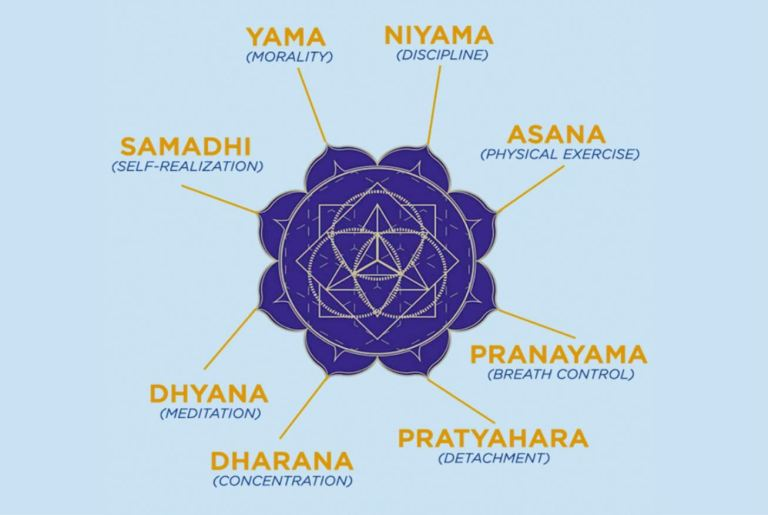
\includegraphics[width=0.6\linewidth,keepaspectratio]{images/yog22}
\end{center}

		\begin{itemize}
		\item Steps progression isn’t meant to be rigid. 
		\item For example, someone might begin the practice of an asana before they have mastered Niyama, still, they must follow the overall elements of the 8 limbs to have a wholesome growth.
		\end{itemize}
		
\end{frame}


%%%%%%%%%%%%%%%%%%%%%%%%%%%%%%%%%%%%%%%%%%%%%%%%%%%%%%%%%%%
\begin{frame}[fragile]\frametitle{Yog}
\begin{sanskrit}
तपःस्वाध्यायेश्वरप्रणिधानानि क्रियायोगः॥१॥
\end{sanskrit}
	\begin{itemize}
	\item Yog 
	\end{itemize}
\end{frame}

%%%%%%%%%%%%%%%%%%%%%%%%%%%%%%%%%%%%%%%%%%%%%%%%%%%%%%%%%%%
\begin{frame}[fragile]\frametitle{Yog}
\begin{sanskrit}
समाधिभावनार्थः क्लेशतनूकरणार्थश्च॥२॥
\end{sanskrit}
	\begin{itemize}
	\item Yog 
	\end{itemize}
\end{frame}



%%%%%%%%%%%%%%%%%%%%%%%%%%%%%%%%%%%%%%%%%%%%%%%%%%%%%%%%%%%
\begin{frame}[fragile]\frametitle{Yog}
\begin{sanskrit}
अविद्यास्मितारागद्वेषाभिनिवेशाः क्लेशाः॥३॥
\end{sanskrit}
	\begin{itemize}
	\item Yog 
	\end{itemize}
\end{frame}

%%%%%%%%%%%%%%%%%%%%%%%%%%%%%%%%%%%%%%%%%%%%%%%%%%%%%%%%%%%
\begin{frame}[fragile]\frametitle{Yog}
\begin{sanskrit}
अविद्याक्षेत्रमुत्तरेषां प्रसुप्ततनुविच्छिन्नोदाराणाम्॥४॥
\end{sanskrit}
	\begin{itemize}
	\item Yog 
	\end{itemize}
\end{frame}


%%%%%%%%%%%%%%%%%%%%%%%%%%%%%%%%%%%%%%%%%%%%%%%%%%%%%%%%%%%
\begin{frame}[fragile]\frametitle{Yog}
\begin{sanskrit}
अनित्याशुचिदुःखानात्मसु नित्यशुचिसुखात्मख्यातिरविद्या॥५॥
\end{sanskrit}
	\begin{itemize}
	\item Yog 
	\end{itemize}
\end{frame}


%%%%%%%%%%%%%%%%%%%%%%%%%%%%%%%%%%%%%%%%%%%%%%%%%%%%%%%%%%%
\begin{frame}[fragile]\frametitle{Yog}
\begin{sanskrit}
दृग्दर्शनशक्त्योरेकात्मतेवास्मिता॥६॥
\end{sanskrit}
	\begin{itemize}
	\item Yog 
	\end{itemize}
\end{frame}



%%%%%%%%%%%%%%%%%%%%%%%%%%%%%%%%%%%%%%%%%%%%%%%%%%%%%%%%%%%
\begin{frame}[fragile]\frametitle{Yog}
\begin{sanskrit}
सुखानुशयी रागः॥७॥
\end{sanskrit}
	\begin{itemize}
	\item Yog 
	\end{itemize}
\end{frame}



%%%%%%%%%%%%%%%%%%%%%%%%%%%%%%%%%%%%%%%%%%%%%%%%%%%%%%%%%%%
\begin{frame}[fragile]\frametitle{Yog}
\begin{sanskrit}
दुःखानुशयी द्वेषः॥८॥
\end{sanskrit}
	\begin{itemize}
	\item Yog 
	\end{itemize}
\end{frame}



%%%%%%%%%%%%%%%%%%%%%%%%%%%%%%%%%%%%%%%%%%%%%%%%%%%%%%%%%%%
\begin{frame}[fragile]\frametitle{Yog}
\begin{sanskrit}
स्वरसवाही विदुषोऽपि तथारूढो भिनिवेशः॥९॥
\end{sanskrit}
	\begin{itemize}
	\item Yog 
	\end{itemize}
\end{frame}


%%%%%%%%%%%%%%%%%%%%%%%%%%%%%%%%%%%%%%%%%%%%%%%%%%%%%%%%%%%
\begin{frame}[fragile]\frametitle{Yog}
\begin{sanskrit}
ते प्रतिप्रसवहेयाः सूक्ष्माः॥१०॥
\end{sanskrit}
	\begin{itemize}
	\item Yog 
	\end{itemize}
\end{frame}


%%%%%%%%%%%%%%%%%%%%%%%%%%%%%%%%%%%%%%%%%%%%%%%%%%%%%%%%%%%
\begin{frame}[fragile]\frametitle{Yog}
\begin{sanskrit}
ध्यानहेयास्तद्वृत्तयः॥११॥
\end{sanskrit}
	\begin{itemize}
	\item Yog 
	\end{itemize}
\end{frame}


%%%%%%%%%%%%%%%%%%%%%%%%%%%%%%%%%%%%%%%%%%%%%%%%%%%%%%%%%%%
\begin{frame}[fragile]\frametitle{Yog}
\begin{sanskrit}
क्लेशमूलः कर्माशयो दृष्टादृष्टजन्मवेदनीयः॥१२॥
\end{sanskrit}
	\begin{itemize}
	\item Yog 
	\end{itemize}
\end{frame}


%%%%%%%%%%%%%%%%%%%%%%%%%%%%%%%%%%%%%%%%%%%%%%%%%%%%%%%%%%%
\begin{frame}[fragile]\frametitle{Yog}
\begin{sanskrit}
सति मूले तद्विपाको जात्यायुर्भोगाः॥१३॥
\end{sanskrit}
	\begin{itemize}
	\item Yog 
	\end{itemize}
\end{frame}


%%%%%%%%%%%%%%%%%%%%%%%%%%%%%%%%%%%%%%%%%%%%%%%%%%%%%%%%%%%
\begin{frame}[fragile]\frametitle{Yog}
\begin{sanskrit}
ते ह्लादपरितापफलाः पुण्यापुण्यहेतुत्वात्॥१४॥
\end{sanskrit}
	\begin{itemize}
	\item Yog 
	\end{itemize}
\end{frame}


%%%%%%%%%%%%%%%%%%%%%%%%%%%%%%%%%%%%%%%%%%%%%%%%%%%%%%%%%%%
\begin{frame}[fragile]\frametitle{Yog}
\begin{sanskrit}
परिणामतापसंस्कारदुःखैर्गुणवृत्तिविरोधाच्च दुःखमेव सर्वं विवेकिनः॥१५॥
\end{sanskrit}
	\begin{itemize}
	\item Yog 
	\end{itemize}
\end{frame}


%%%%%%%%%%%%%%%%%%%%%%%%%%%%%%%%%%%%%%%%%%%%%%%%%%%%%%%%%%%
\begin{frame}[fragile]\frametitle{Yog}
\begin{sanskrit}
हेयं दुःखमनागतम्॥१६॥
\end{sanskrit}
	\begin{itemize}
	\item Yog 
	\end{itemize}
\end{frame}


%%%%%%%%%%%%%%%%%%%%%%%%%%%%%%%%%%%%%%%%%%%%%%%%%%%%%%%%%%%
\begin{frame}[fragile]\frametitle{Yog}
\begin{sanskrit}
द्रष्टृदृश्ययोः संयोगो हेयहेतुः॥१७॥
\end{sanskrit}
	\begin{itemize}
	\item Yog 
	\end{itemize}
\end{frame}

%%%%%%%%%%%%%%%%%%%%%%%%%%%%%%%%%%%%%%%%%%%%%%%%%%%%%%%%%%%
\begin{frame}[fragile]\frametitle{Yog}
\begin{sanskrit}
प्रकाशक्रियास्थितिशीलं भूतेन्द्रियात्मकं भोगापवर्गार्थं दृश्यम्॥१८॥
\end{sanskrit}
	\begin{itemize}
	\item Yog 
	\end{itemize}
\end{frame}


%%%%%%%%%%%%%%%%%%%%%%%%%%%%%%%%%%%%%%%%%%%%%%%%%%%%%%%%%%%
\begin{frame}[fragile]\frametitle{Yog}
\begin{sanskrit}
विशेषाविशेषलिङ्गमात्रालिङ्गानि गुणपर्वाणि॥१९॥
\end{sanskrit}
	\begin{itemize}
	\item Yog 
	\end{itemize}
\end{frame}

%%%%%%%%%%%%%%%%%%%%%%%%%%%%%%%%%%%%%%%%%%%%%%%%%%%%%%%%%%%
\begin{frame}[fragile]\frametitle{Yog}
\begin{sanskrit}
द्रष्टा दृशिमात्रः शुद्धोऽपि प्रत्ययानुपश्यः॥२०॥
\end{sanskrit}
	\begin{itemize}
	\item Yog 
	\end{itemize}
\end{frame}


%%%%%%%%%%%%%%%%%%%%%%%%%%%%%%%%%%%%%%%%%%%%%%%%%%%%%%%%%%%
\begin{frame}[fragile]\frametitle{Yog}
\begin{sanskrit}
तदर्थ एव दृश्यस्यात्मा॥२१॥
\end{sanskrit}
	\begin{itemize}
	\item Yog 
	\end{itemize}
\end{frame}


%%%%%%%%%%%%%%%%%%%%%%%%%%%%%%%%%%%%%%%%%%%%%%%%%%%%%%%%%%%
\begin{frame}[fragile]\frametitle{Yog}
\begin{sanskrit}
कृतार्थं प्रति नष्टमप्यनष्टं तदन्यसाधारणत्वात्॥२२॥
\end{sanskrit}
	\begin{itemize}
	\item Yog 
	\end{itemize}
\end{frame}


%%%%%%%%%%%%%%%%%%%%%%%%%%%%%%%%%%%%%%%%%%%%%%%%%%%%%%%%%%%
\begin{frame}[fragile]\frametitle{Yog}
\begin{sanskrit}
स्वस्वामिशक्त्योः स्वरूपोपलब्धिहेतुः संयोगः॥२३॥
\end{sanskrit}
	\begin{itemize}
	\item Yog 
	\end{itemize}
\end{frame}

%%%%%%%%%%%%%%%%%%%%%%%%%%%%%%%%%%%%%%%%%%%%%%%%%%%%%%%%%%%
\begin{frame}[fragile]\frametitle{Yog}
\begin{sanskrit}
तस्य हेतुरविद्या॥२४॥
\end{sanskrit}
	\begin{itemize}
	\item Yog 
	\end{itemize}
\end{frame}

%%%%%%%%%%%%%%%%%%%%%%%%%%%%%%%%%%%%%%%%%%%%%%%%%%%%%%%%%%%
\begin{frame}[fragile]\frametitle{Yog}
\begin{sanskrit}
तदभावात् संयोगाभावो हानं तद् दृशेः कैवल्यम्॥२५॥
\end{sanskrit}
	\begin{itemize}
	\item Yog 
	\end{itemize}
\end{frame}

%%%%%%%%%%%%%%%%%%%%%%%%%%%%%%%%%%%%%%%%%%%%%%%%%%%%%%%%%%%
\begin{frame}[fragile]\frametitle{Yog}
\begin{sanskrit}
विवेकख्यातिरविप्लवा हानोपायः॥२६॥
\end{sanskrit}
	\begin{itemize}
	\item Yog 
	\end{itemize}
\end{frame}

%%%%%%%%%%%%%%%%%%%%%%%%%%%%%%%%%%%%%%%%%%%%%%%%%%%%%%%%%%%
\begin{frame}[fragile]\frametitle{Yog}
\begin{sanskrit}
तस्य सप्तधा प्रान्तभूमिः प्रज्ञा॥२७॥
\end{sanskrit}
	\begin{itemize}
	\item Yog 
	\end{itemize}
\end{frame}


%%%%%%%%%%%%%%%%%%%%%%%%%%%%%%%%%%%%%%%%%%%%%%%%%%%%%%%%%%%
\begin{frame}[fragile]\frametitle{Yog}
\begin{sanskrit}
योगाङ्गाऽनुष्ठानादशुद्धिक्षये ज्ञानदीप्तिराविवेकख्यातेः॥२८॥
\end{sanskrit}
	\begin{itemize}
	\item Yog 
	\end{itemize}
\end{frame}

%%%%%%%%%%%%%%%%%%%%%%%%%%%%%%%%%%%%%%%%%%%%%%%%%%%%%%%%%%%
\begin{frame}[fragile]\frametitle{Yog}
\begin{sanskrit}
यमनियमासनप्राणायामप्रत्याहारधारणाध्यानसमाधयोऽष्टावङ्गानि॥२९॥
\end{sanskrit}
	\begin{itemize}
	\item Yog 
	\end{itemize}
\end{frame}


%%%%%%%%%%%%%%%%%%%%%%%%%%%%%%%%%%%%%%%%%%%%%%%%%%%%%%%%%%%
\begin{frame}[fragile]\frametitle{Yog}
\begin{sanskrit}
अहिंसासत्यास्तेयब्रह्मचर्यापरिग्रहा यमाः॥३०॥
\end{sanskrit}
	\begin{itemize}
	\item Yog 
	\end{itemize}
\end{frame}


%%%%%%%%%%%%%%%%%%%%%%%%%%%%%%%%%%%%%%%%%%%%%%%%%%%%%%%%%%%
\begin{frame}[fragile]\frametitle{Yog}
\begin{sanskrit}
जातिदेशकालसमयानवच्छिन्नाः सार्वभौमा महाव्रतम्॥३१॥
\end{sanskrit}
	\begin{itemize}
	\item Yog 
	\end{itemize}
\end{frame}



%%%%%%%%%%%%%%%%%%%%%%%%%%%%%%%%%%%%%%%%%%%%%%%%%%%%%%%%%%%
\begin{frame}[fragile]\frametitle{Yog}
\begin{sanskrit}
शौचसंतोषतपःस्वाध्यायेश्वरप्रणिधानानि नियमाः॥३२॥
\end{sanskrit}
	\begin{itemize}
	\item Yog 
	\end{itemize}
\end{frame}


%%%%%%%%%%%%%%%%%%%%%%%%%%%%%%%%%%%%%%%%%%%%%%%%%%%%%%%%%%%
\begin{frame}[fragile]\frametitle{Yog}
\begin{sanskrit}
वितर्कबाधने प्रतिपक्षभावनम्॥३३॥
\end{sanskrit}
	\begin{itemize}
	\item Yog 
	\end{itemize}
\end{frame}



%%%%%%%%%%%%%%%%%%%%%%%%%%%%%%%%%%%%%%%%%%%%%%%%%%%%%%%%%%%
\begin{frame}[fragile]\frametitle{Yog}
\begin{sanskrit}
वितर्का हिंसादयः कृतकारितानुमोदिता लोभक्रोधमोहपूर्वका मृदुमध्याधिमात्रा दुःखाज्ञानानन्तफला इति प्रतिपक्षभावनम्॥३४॥
\end{sanskrit}
	\begin{itemize}
	\item Yog 
	\end{itemize}
\end{frame}

%%%%%%%%%%%%%%%%%%%%%%%%%%%%%%%%%%%%%%%%%%%%%%%%%%%%%%%%%%%
\begin{frame}[fragile]\frametitle{Yog}
\begin{sanskrit}
अहिंसाप्रतिष्ठायां तत्सन्निधौ वैरत्यागः॥३५॥
\end{sanskrit}
	\begin{itemize}
	\item Yog 
	\end{itemize}
\end{frame}


%%%%%%%%%%%%%%%%%%%%%%%%%%%%%%%%%%%%%%%%%%%%%%%%%%%%%%%%%%%
\begin{frame}[fragile]\frametitle{Yog}
\begin{sanskrit}
सत्यप्रतिष्ठायां क्रियाफलाश्रयत्वम्॥३६॥
\end{sanskrit}
	\begin{itemize}
	\item Yog 
	\end{itemize}
\end{frame}


%%%%%%%%%%%%%%%%%%%%%%%%%%%%%%%%%%%%%%%%%%%%%%%%%%%%%%%%%%%
\begin{frame}[fragile]\frametitle{Yog}
\begin{sanskrit}
अस्तेयप्रतिष्ठायां सर्वरत्नोपस्थानम्॥३७॥
\end{sanskrit}
	\begin{itemize}
	\item Yog 
	\end{itemize}
\end{frame}


%%%%%%%%%%%%%%%%%%%%%%%%%%%%%%%%%%%%%%%%%%%%%%%%%%%%%%%%%%%
\begin{frame}[fragile]\frametitle{Yog}
\begin{sanskrit}
ब्रह्मचर्यप्रतिष्ठायां वीर्यलाभः॥३८॥
\end{sanskrit}
	\begin{itemize}
	\item Yog 
	\end{itemize}
\end{frame}


%%%%%%%%%%%%%%%%%%%%%%%%%%%%%%%%%%%%%%%%%%%%%%%%%%%%%%%%%%%
\begin{frame}[fragile]\frametitle{Yog}
\begin{sanskrit}
अपरिग्रहस्थैर्ये जन्मकथंतासंबोधः॥३९॥
\end{sanskrit}
	\begin{itemize}
	\item Yog 
	\end{itemize}
\end{frame}



%%%%%%%%%%%%%%%%%%%%%%%%%%%%%%%%%%%%%%%%%%%%%%%%%%%%%%%%%%%
\begin{frame}[fragile]\frametitle{Yog}
\begin{sanskrit}
शौचात् स्वाङ्गजुगुप्सा परैरसंसर्गः॥४०॥
\end{sanskrit}
	\begin{itemize}
	\item Yog 
	\end{itemize}
\end{frame}



%%%%%%%%%%%%%%%%%%%%%%%%%%%%%%%%%%%%%%%%%%%%%%%%%%%%%%%%%%%
\begin{frame}[fragile]\frametitle{Yog}
\begin{sanskrit}
सत्त्वशुद्धिसौमनस्यैकाग्र्येन्द्रियजयात्मदर्शनयोग्यत्वानि च॥४१॥
\end{sanskrit}
	\begin{itemize}
	\item Yog 
	\end{itemize}
\end{frame}


%%%%%%%%%%%%%%%%%%%%%%%%%%%%%%%%%%%%%%%%%%%%%%%%%%%%%%%%%%%
\begin{frame}[fragile]\frametitle{Yog}
\begin{sanskrit}
संतोषादनुत्तमसुखलाभः॥४२॥
\end{sanskrit}
	\begin{itemize}
	\item Yog 
	\end{itemize}
\end{frame}


%%%%%%%%%%%%%%%%%%%%%%%%%%%%%%%%%%%%%%%%%%%%%%%%%%%%%%%%%%%
\begin{frame}[fragile]\frametitle{Yog}
\begin{sanskrit}
कायेन्द्रियसिद्धिरशुद्धिक्षयात्तपसः॥४३॥
\end{sanskrit}
	\begin{itemize}
	\item Yog 
	\end{itemize}
\end{frame}


%%%%%%%%%%%%%%%%%%%%%%%%%%%%%%%%%%%%%%%%%%%%%%%%%%%%%%%%%%%
\begin{frame}[fragile]\frametitle{Yog}
\begin{sanskrit}
स्वाध्यायादिष्टदेवतासंप्रयोगः॥४४॥
\end{sanskrit}
	\begin{itemize}
	\item Yog 
	\end{itemize}
\end{frame}


%%%%%%%%%%%%%%%%%%%%%%%%%%%%%%%%%%%%%%%%%%%%%%%%%%%%%%%%%%%
\begin{frame}[fragile]\frametitle{Yog}
\begin{sanskrit}
समाधिसिद्धिरीश्वरप्रणिधानात्॥४५॥
\end{sanskrit}
	\begin{itemize}
	\item Yog 
	\end{itemize}
\end{frame}


%%%%%%%%%%%%%%%%%%%%%%%%%%%%%%%%%%%%%%%%%%%%%%%%%%%%%%%%%%%
\begin{frame}[fragile]\frametitle{Yog}
\begin{sanskrit}
स्थिरसुखमासनम्॥४६॥
\end{sanskrit}
	\begin{itemize}
	\item Yog 
	\end{itemize}
\end{frame}


%%%%%%%%%%%%%%%%%%%%%%%%%%%%%%%%%%%%%%%%%%%%%%%%%%%%%%%%%%%
\begin{frame}[fragile]\frametitle{Yog}
\begin{sanskrit}
प्रयत्नशैथिल्यानन्त्यसमापत्तिभ्याम्॥४७॥
\end{sanskrit}
	\begin{itemize}
	\item Yog 
	\end{itemize}
\end{frame}

%%%%%%%%%%%%%%%%%%%%%%%%%%%%%%%%%%%%%%%%%%%%%%%%%%%%%%%%%%%
\begin{frame}[fragile]\frametitle{Yog}
\begin{sanskrit}
ततो द्वन्द्वानभिघातः॥४८॥
\end{sanskrit}
	\begin{itemize}
	\item Yog 
	\end{itemize}
\end{frame}


%%%%%%%%%%%%%%%%%%%%%%%%%%%%%%%%%%%%%%%%%%%%%%%%%%%%%%%%%%%
\begin{frame}[fragile]\frametitle{Yog}
\begin{sanskrit}
तस्मिन् सति श्वासप्रश्वासयोर्गतिविच्छेदः प्राणायामः॥४९॥
\end{sanskrit}
	\begin{itemize}
	\item Yog 
	\end{itemize}
\end{frame}



%%%%%%%%%%%%%%%%%%%%%%%%%%%%%%%%%%%%%%%%%%%%%%%%%%%%%%%%%%%
\begin{frame}[fragile]\frametitle{Yog}
\begin{sanskrit}
बाह्याभ्यन्तरस्तम्भवृत्तिर्देशकालसंख्याभिः परिदृष्टो दीर्घसूक्ष्मः॥५०॥
\end{sanskrit}
	\begin{itemize}
	\item Yog 
	\end{itemize}
\end{frame}


%%%%%%%%%%%%%%%%%%%%%%%%%%%%%%%%%%%%%%%%%%%%%%%%%%%%%%%%%%%
\begin{frame}[fragile]\frametitle{Yog}
\begin{sanskrit}
बाह्याभ्यन्तरविषयाक्षेपी चतुर्थः॥५१॥
\end{sanskrit}
	\begin{itemize}
	\item Yog 
	\end{itemize}
\end{frame}

%%%%%%%%%%%%%%%%%%%%%%%%%%%%%%%%%%%%%%%%%%%%%%%%%%%%%%%%%%%
\begin{frame}[fragile]\frametitle{Yog}
\begin{sanskrit}
ततः क्षीयते प्रकाशावरणम्॥५२॥
\end{sanskrit}
	\begin{itemize}
	\item Yog 
	\end{itemize}
\end{frame}

%%%%%%%%%%%%%%%%%%%%%%%%%%%%%%%%%%%%%%%%%%%%%%%%%%%%%%%%%%%
\begin{frame}[fragile]\frametitle{Yog}
\begin{sanskrit}
धारणासु च योग्यता मनसः॥५३॥
\end{sanskrit}
	\begin{itemize}
	\item Yog 
	\end{itemize}
\end{frame}

%%%%%%%%%%%%%%%%%%%%%%%%%%%%%%%%%%%%%%%%%%%%%%%%%%%%%%%%%%%
\begin{frame}[fragile]\frametitle{Yog}
\begin{sanskrit}
स्वविषयासंप्रयोगे चित्तस्य स्वरूपानुकार इवेन्द्रियाणां प्रत्याहारः॥५४॥
\end{sanskrit}
	\begin{itemize}
	\item Yog 
	\end{itemize}
\end{frame}

%%%%%%%%%%%%%%%%%%%%%%%%%%%%%%%%%%%%%%%%%%%%%%%%%%%%%%%%%%%
\begin{frame}[fragile]\frametitle{Yog}
\begin{sanskrit}
ततः परमा वश्यतेन्द्रियाणाम्॥५५॥
\end{sanskrit}
	\begin{itemize}
	\item Yog 
	\end{itemize}
\end{frame}

